%Notes by Harsh Mistry 
%CS 246
%based on Template from : https://www.cs.cmu.edu/~ggordon/10725-F12/template.tex

\documentclass{article}
\setlength{\oddsidemargin}{0.25 in}
\setlength{\evensidemargin}{-0.25 in}
\setlength{\topmargin}{-0.6 in}
\setlength{\textwidth}{6.5 in}
\setlength{\textheight}{8.5 in}
\setlength{\headsep}{0.75 in}
\setlength{\parindent}{0 in}
\setlength{\parskip}{0.1 in}
\usepackage{amsfonts,graphicx, amssymb}
\usepackage[fleqn]{amsmath}
\usepackage{fixltx2e}
\usepackage{color}
\usepackage{tcolorbox}
\usepackage{graphicx}
\graphicspath{ {images/} }
\usepackage{lipsum}
\usepackage{listings}
\usepackage{scrextend}
\tcbuselibrary{skins,breakable}
\usetikzlibrary{shadings,shadows}
\newcounter{lecnum}
\renewcommand{\thepage}{\thelecnum-\arabic{page}}
\renewcommand{\thesection}{\thelecnum.\arabic{section}}
\renewcommand{\theequation}{\thelecnum.\arabic{equation}}
\renewcommand{\thefigure}{\thelecnum.\arabic{figure}}
\renewcommand{\thetable}{\thelecnum.\arabic{table}}
\newcommand{\lecture}[4]{
   \pagestyle{myheadings}
   \thispagestyle{plain}
   \newpage
   \setcounter{lecnum}{#1}
   \setcounter{page}{1}
   
   
%Info Box 
   \begin{center}
   \framebox{
      \vbox{\vspace{2mm}
    \hbox to 6.28in { {\bf CS 246 - Object Oriented Programming  
	\hfill Fall 2016} }
       \vspace{4mm}
       \hbox to 6.28in { {\Large \hfill Lecture #1: #2  \hfill} }
       \vspace{2mm}
       \hbox to 6.28in { {\it Lecturer: #3 \hfill Notes By: #4} }
      \vspace{2mm}}
   }
   \end{center}
   
   \markboth{Lecture #1: #2}{Lecture #1: #2}



 
}

\renewcommand{\cite}[1]{[#1]}
\def\beginrefs{\begin{list}%
        {[\arabic{equation}]}{\usecounter{equation}
         \setlength{\leftmargin}{2.0truecm}\setlength{\labelsep}{0.4truecm}%
         \setlength{\labelwidth}{1.6truecm}}}
\def\endrefs{\end{list}}
\def\bibentry#1{\item[\hbox{[#1]}]}

\newcommand{\fig}[3]{
			\vspace{#2}
			\begin{center}
			Figure \thelecnum.#1:~#3
			\end{center}
	}
	
\newcommand{\pipe}{\(\mid\)}
\newcommand{\ctr}{\(\wedge\)}

\newtheorem{theorem}{Theorem}[lecnum]
\newtheorem{lemma}[theorem]{Lemma}
\newtheorem{ex}[theorem]{Example}
\newtheorem{proposition}[theorem]{Proposition}
\newtheorem{claim}[theorem]{Claim}
\newtheorem{corollary}[theorem]{Corollary}
\newtheorem{definition}[theorem]{Definition}
\newenvironment{proof}{{\bf Proof:}}{\hfill\rule{2mm}{2mm}}
\newcommand\E{\mathbb{E}}

%color definitions :
\definecolor{darkred}{rgb}{0.55, 0.0, 0.0}
\definecolor{lightcoral}{rgb}{0.94, 0.5, 0.5}
\definecolor{tomato}{rgb}{1.0, 0.39, 0.28}
\definecolor{lightgray}{rgb}{.9,.9,.9}
\definecolor{darkgray}{rgb}{.4,.4,.4}
\definecolor{purple}{rgb}{0.65, 0.12, 0.82}
\definecolor{lightgreen}{rgb}{0.56, 0.93, 0.56}
\definecolor{darkgreen}{rgb}{0.0, 0.2, 0.13}
\definecolor{limegreen}{rgb}{0.2, 0.8, 0.2}
\definecolor{lightblue}{rgb}{0.68, 0.85, 0.9}
\definecolor{darkblue}{rgb}{0.0, 0.0, 0.55}


%Environments
\newenvironment{exblock}[1]{%
    \tcolorbox[beamer,%
    noparskip,breakable,
    colback=lightgreen,colframe=darkgreen,%
    colbacklower=limegreen!75!lightgreen,%
    title=#1]}%
    {\endtcolorbox}

\newenvironment{ablock}[1]{%
    \tcolorbox[beamer,%
    noparskip,breakable,
    colback=lightcoral,colframe=darkred,%
    colbacklower=tomato!75!lightcoral,%
    title=#1]}%
    {\endtcolorbox}

\newenvironment{cblock}[1]{%
    \tcolorbox[beamer,%
    noparskip,breakable,
    colback=lightblue,colframe=darkblue,%
    colbacklower=darkblue!75!lightblue,%
    title=#1]}%
    {\endtcolorbox}


%Languages
\lstdefinelanguage{JavaScript}{
  keywords={typeof, new, true, false, catch, function, return, null, catch, switch, var, if, in,  fi, while, do, else, case, break, const},
  keywordstyle=\color{blue}\bfseries,
  ndkeywords={class, export, boolean, throw, implements, import, this, struct},
  ndkeywordstyle=\color{darkgray}\bfseries,
  identifierstyle=\color{black},
  sensitive=false,
  comment=[l]{//},
  morecomment=[s]{/*}{*/},
  commentstyle=\color{purple}\ttfamily,
  stringstyle=\color{red}\ttfamily,
  morestring=[b]',
  morestring=[b]"
}

%Listings
\lstset{
   language=JavaScript,
   backgroundcolor=\color{lightgray},
   extendedchars=true,
   basicstyle=\footnotesize\ttfamily,
   showstringspaces=false,
   showspaces=false,
   numbers=left,
   numberstyle=\footnotesize,
   numbersep=9pt,
   tabsize=2,
   breaklines=true,
   showtabs=false,
   captionpos=b
}


%Start of Document 
\begin{document}

\lecture{10}{November 17, 2016}{Brad Lushman}{Harsh Mistry}

\section{Visitor Pattern}
The visitor pattern is often used to implementing a concept called \textbf{double dispatch}.
Using this method, we can implement a program where action can be based upon two different objects.To achieve this goal we can combine overriding and overloading.

\begin{ex} Basic video game with enemies and weapons using the visitor pattern\\
\begin{center}
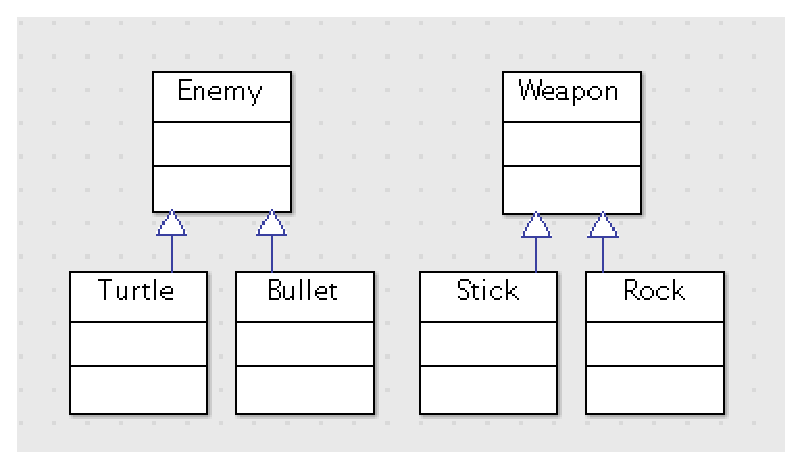
\includegraphics[scale=0.8]{lec10-1}
\end{center}

We want a different action to occur when different weapons are used on different enemies. So we introduce a overloaded strike method.

\begin{lstlisting}
class Enemy{
		virtual void beStruckBy(Weapon &w) = 0;
};

class Turtle : public Enemy{
		void beStruckBy(Weapon &w) override {
			w.strike(*this); 
		}
}

class Bullet : public Enemy {
		void beStruckBy(Weapon &w) override{
			w.strike(*this); //Different then previous subclass, due to different parameter types of *this
		}
};

class Weapon {
		//Overloads
		virtual void strike(Turtle &t) = 0;
		virtual void strike(Bullet &t)  = 0;
};

class  Stick : public Weapon{
		void strike (Turtle &t) override {
			//Strike turtle with stick 
		}
		
		void strike (Bullet &t) override {
			//Strike bullet with stick 
		}
};

class Rock : Weapon {
		void strike (Turtle &t) override {
			//Strike turtle with rock 
		}
		
		void strike (Bullet &t) override {
			//Strike bullet with rock
		}
}; 

//Client Code
Enemy *e = new Bullet(...);
Enemy *w = new Rock(...);

e->beStructBy(w);

\end{lstlisting}
\end{ex}

Visitor pattern can also be used to add functionality to existing classes without changing or recompiling them.

\begin{ex} Adding a visitor to the book hierarchy\\
\begin{lstlisting}
class Book{
	public:
		virtual void accept (BookVisitor &v) {v.visit(*this);}
};

class Text : public Book {
		Void accept (BookVisitor &v)  override {v.vist(*this);}
};

class BookVisitor{
		virtual void visit (Book &b) = 0;
		virtual void visit (Text &b) = 0;
		virtual void visit (Comic &b) = 0;
}

// Now we want to Track how many of each type of book is available
// - Books are sorted by author
// - Texts are sorted by topic 
// - Comics are sorted by hero
// This can be done using a map<string, int>

class Catalogue : BookVisitor {
		map<string, int> theCatalogue;
	public :
		map<string, int> getResult() {return theCatalogue;}
		void visit (Book &b) override { ++ theCatalogue[b.getAuthor()];}
		void visit (Text &t) override { ++theCatalogue[t.getTopic()];}
		void visit (Comic &t) override { ++theCatalogue[t.getHero()];}
};
\end{lstlisting}
\end{ex}

\section{Compilation Dependencies - include vs forward declare}
Consider : 
\begin{lstlisting}
Class A {...};
Class B : public A { ...}
Class C {
		A myA();
};
Class D {
		A *myAP
};
Class E {
		A f(A a);
};
\end{lstlisting}

\begin{itemize}
\item Class B and C require include statements as the compiler needs to know more information about A before it can allocate the necessary space and construct the fields. 

\item Class D and E do not require include statements as the size of A does not need to be known to construct the object. 
\end{itemize}

In addition, the implementations of each object can require the use of include statements, as the actual definition may require more information on additional classes. If this is the case, write the include within the .cc file, as it can never be apart of the include cycle. 

So, If there is no compilation dependency necessitated by the code, \textbf{DO NOT} create one with unnecessary includes. 

Now Consider the XWindow class : 
\begin{lstlisting}
Class XWindow {
		Display *d;
		Window w;
		int s;
		Gc gc;
		unsigned long colours [10];
	public :
		...
};
\end{lstlisting}

If any of the private data fields were to change, all clients must recompile. To  avoid having to recompile the client, we can use the \textbf{pimpl idom} (Pointer to implementation) .

\begin{lstlisting}
//Included Header (Window.h)
Class XWindowInput; //Forward Declaration

Class XWindow {
		XWindowInput *pimpl;
	public :
		...
};

//Separate Header File (xwindowImpl.h)
#include(X11/Xlib.h)

struct XWindowImpl{
		Display *d;
		Window *d;
		window q;
		int s;
		GC gc;
		unsigned long colours[10];
};

//Window.cc
#include "window.h"
#include "xwindowImpl.h"

Xwindow::Xwindow(): pimpl{new XWindowInpml {...{ } {...} 

//In other methods replace d, w, s, etc with pimpl->d, pimpl->w, ...
\end{lstlisting}

If you confine all private fields to XWindowImpl, only window.cc needs to be recompiled if you change XWindow's implementation. 

\textbf{Generalization :} If there is multiple X window implementations, then we can make the Impl struct a superclass

\begin{center}
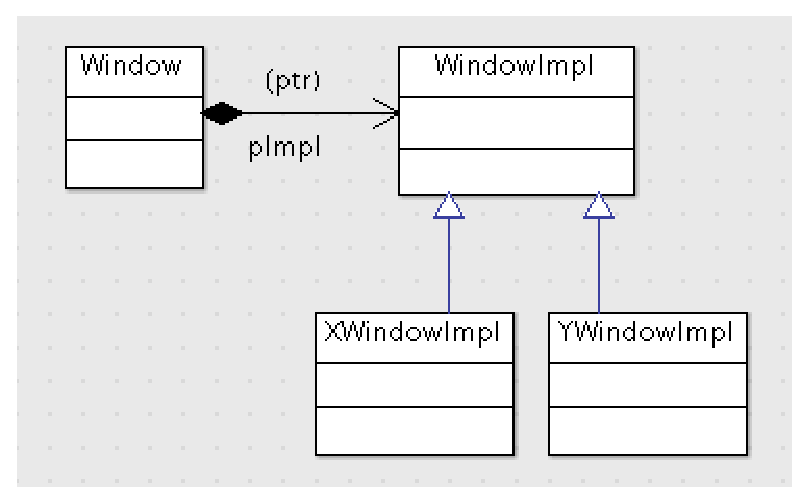
\includegraphics[scale=0.8]{lec10-2}
\end{center}

Implementing a class hierarchy with implementations is called the \textbf{Bridge Pattern}.

\section{Measuring of Design Quality}
\subsection{Coupling and Cohesion }
\begin{itemize}
\item Coupling : Coupling is the degree to which distinct modules depend on each other 
\begin{itemize}
\item Low Coupling 
\begin{itemize}
\item Modules communicate via function calls with basic parameters and results
\end{itemize} 
\item Relative Amount of Coupling 
\begin{itemize}
\item Modules pass array/structs back and forth
\item Modules affect each other's control flow
\item Modules share global data
\end{itemize}
\item High Coupling
\begin{itemize}
\item Modules have access to each other's implementations (friends)
\end{itemize}
\end{itemize}


\item Cohesion : Cohesion is how closely elements of the module are related to each other 
\begin{itemize}
\item Low Cohesion 
\begin{itemize}
\item Arbitrary grouping of unrelated elements (e.g \verb|<utility>|) 
\end{itemize}
\item Relative Amount of Cohesion
\begin{itemize}
\item Elements share a common theme, but are otherwise unrelated. Perhaps also share some base code (e.g \verb|<algorithm>|)
\item Elements manipulate state over the lifetime of an object (e.g \verb|open/read/close| files)
\item Elements pass data to each other 
\end{itemize}
\item High Cohesion 
\begin{itemize}
\item Elements cooperate to perform exactly one task. 
\end{itemize}
\end{itemize}
\end{itemize}

High coupling implies changes to one module requires changes to be made to other modules. This results in a implementation that is harder to reuse. 

Low cohesion implies poorly orginized code and make its hard for the client to complete task and include classes which may not be needed. 

Ultimately the goal is to have low coupling and high cohesion. 
 
\subsection{Decoupling the Interface (MVC)}
Primary program classes should not be printing things. 

\begin{ex}  Bad Design Example 
\begin{lstlisting}
class ChessBoard { 
		...
		cout <<< "Your move" << endl;
};
\end{lstlisting}
\end{ex}

Example 10.3 is a bad design habit as it ties the output to cout and prevents you from reusing the class for other purposes.

One solution is to give the class stream objects with which it can do Input/Output operations. 
\begin{lstlisting}
Class ChessBoard{
		std::istream &in;
		std::ostream &out;
	public : 
		ChessBoard(std::istream &i, std::ostream &o) : in{i}, out{o} {} 
		
		...
		out << "your move" << endl;
};
\end{lstlisting}

This solution works, but still limits you to text output and prevents you from implementing different types of outputs (i.e different languages). A better implementation is to have the class not communicate at all.  

\textbf{Single Responsibility Principle : } "A class should have only one reason to change."

In essence, the idea for communicating with the chess board without printing is to simply make use of parameters and results. So , ensure use communication is excluded from main program classes. 

Expanding further, main should not be used either to communicate with the user, as main is difficult to reuse. Ideally, main should be fairly short and a separate class should be used to handle communication.  This idea is known as the \textbf{Model-View-Controller Pattern (MVC)}.

The goal of MVC is to separate out the distinct portions of the application 
\begin{itemize}
\item Model - Data you are manipulating (e.g game state) 
\begin{itemize}
\item Can have multiple views 
\item Classic observer pattern if you choose to communicate with the view directly
\end{itemize}
\item View - How the model is displayed to the user 
\begin{itemize}
\item Indicates control flow through model and view
\item May encapsulate data
\item May fetch user input 
\end{itemize}
\item Controller - How the model is manipulated. 
\end{itemize}
\begin{center}
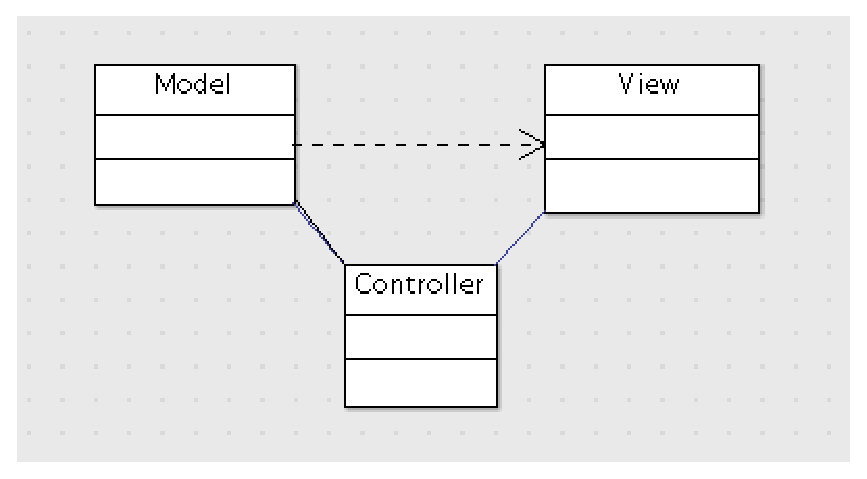
\includegraphics[scale=0.8]{lec10-3}
\end{center}


\section{Exceptions Safety}
Consider : 
\begin{lstlisting}
void f() {
	MyClass *p =  new MyClass;
	MyClass mc;
	g();
	delete p;
}
\end{lstlisting}

Within the example there are no leaks, but if g() raises an exception there may be leaks. During stack unwinding all stack allocated data is cleaned up, but heap allocated memory is not destroy.  So, within the example, p would be leaked. 

A better implementation : 
\begin{lstlisting}
void f() {
	MyClass *p =  new MyClass;
	MyClass mc;
	try {
		g();
	}
	catch (...) {
		delete p;
		throw; 
	}
	
	delete p;
}
\end{lstlisting}

The above implementation works, but involved code duplication. In some languages, there is a "finally" clauses. Unfortunately, C++ is not one of those languages.  In c++ the only thing you can count on in c++ is that destructor for stack allocated data will run. So, use stack allocated data as much as possible and use this to your advantage. 

This leads to the popular c++ idiom : \textbf{RAII - Resource Acquisition is Initialization}. RAII states that every resource should be wrapped in a stack-allocated object whose destructor frees it. 

\begin{lstlisting}
ifstream f {name}; 
//The file is guaranteed to be released when f is popped from the stack (f's destructor is run)
\end{lstlisting}

This concept, can be applied to delete any heap allocated data by using \verb|class std::unique_ptr <t>| which takes a T* in the constructor and will delete the pointer when the item is popped from the stack.

So an ideal implementation for the example with g() would be : 
\begin{lstlisting}
void f() { 
	auto p = std::make_unique<MyClass> ();
	MyClass mc;
	g();
}	
\end{lstlisting}
\end{document}











